\documentclass[twoside]{book}

% Packages required by doxygen
\usepackage{fixltx2e}
\usepackage{calc}
\usepackage{doxygen}
\usepackage[export]{adjustbox} % also loads graphicx
\usepackage{graphicx}
\usepackage[utf8]{inputenc}
\usepackage{makeidx}
\usepackage{multicol}
\usepackage{multirow}
\PassOptionsToPackage{warn}{textcomp}
\usepackage{textcomp}
\usepackage[nointegrals]{wasysym}
\usepackage[table]{xcolor}

% Font selection
\usepackage[T1]{fontenc}
\usepackage[scaled=.90]{helvet}
\usepackage{courier}
\usepackage{amssymb}
\usepackage{sectsty}
\renewcommand{\familydefault}{\sfdefault}
\allsectionsfont{%
  \fontseries{bc}\selectfont%
  \color{darkgray}%
}
\renewcommand{\DoxyLabelFont}{%
  \fontseries{bc}\selectfont%
  \color{darkgray}%
}
\newcommand{\+}{\discretionary{\mbox{\scriptsize$\hookleftarrow$}}{}{}}

% Page & text layout
\usepackage{geometry}
\geometry{%
  a4paper,%
  top=2.5cm,%
  bottom=2.5cm,%
  left=2.5cm,%
  right=2.5cm%
}
\tolerance=750
\hfuzz=15pt
\hbadness=750
\setlength{\emergencystretch}{15pt}
\setlength{\parindent}{0cm}
\setlength{\parskip}{3ex plus 2ex minus 2ex}
\makeatletter
\renewcommand{\paragraph}{%
  \@startsection{paragraph}{4}{0ex}{-1.0ex}{1.0ex}{%
    \normalfont\normalsize\bfseries\SS@parafont%
  }%
}
\renewcommand{\subparagraph}{%
  \@startsection{subparagraph}{5}{0ex}{-1.0ex}{1.0ex}{%
    \normalfont\normalsize\bfseries\SS@subparafont%
  }%
}
\makeatother

% Headers & footers
\usepackage{fancyhdr}
\pagestyle{fancyplain}
\fancyhead[LE]{\fancyplain{}{\bfseries\thepage}}
\fancyhead[CE]{\fancyplain{}{}}
\fancyhead[RE]{\fancyplain{}{\bfseries\leftmark}}
\fancyhead[LO]{\fancyplain{}{\bfseries\rightmark}}
\fancyhead[CO]{\fancyplain{}{}}
\fancyhead[RO]{\fancyplain{}{\bfseries\thepage}}
\fancyfoot[LE]{\fancyplain{}{}}
\fancyfoot[CE]{\fancyplain{}{}}
\fancyfoot[RE]{\fancyplain{}{\bfseries\scriptsize Generated by Doxygen }}
\fancyfoot[LO]{\fancyplain{}{\bfseries\scriptsize Generated by Doxygen }}
\fancyfoot[CO]{\fancyplain{}{}}
\fancyfoot[RO]{\fancyplain{}{}}
\renewcommand{\footrulewidth}{0.4pt}
\renewcommand{\chaptermark}[1]{%
  \markboth{#1}{}%
}
\renewcommand{\sectionmark}[1]{%
  \markright{\thesection\ #1}%
}

% Indices & bibliography
\usepackage{natbib}
\usepackage[titles]{tocloft}
\setcounter{tocdepth}{3}
\setcounter{secnumdepth}{5}
\makeindex

% Hyperlinks (required, but should be loaded last)
\usepackage{ifpdf}
\ifpdf
  \usepackage[pdftex,pagebackref=true]{hyperref}
\else
  \usepackage[ps2pdf,pagebackref=true]{hyperref}
\fi
\hypersetup{%
  colorlinks=true,%
  linkcolor=blue,%
  citecolor=blue,%
  unicode%
}

% Custom commands
\newcommand{\clearemptydoublepage}{%
  \newpage{\pagestyle{empty}\cleardoublepage}%
}

\usepackage{caption}
\captionsetup{labelsep=space,justification=centering,font={bf},singlelinecheck=off,skip=4pt,position=top}

%===== C O N T E N T S =====

\begin{document}

% Titlepage & ToC
\hypersetup{pageanchor=false,
             bookmarksnumbered=true,
             pdfencoding=unicode
            }
\pagenumbering{roman}
\begin{titlepage}
\vspace*{7cm}
\begin{center}%
{\Large My Project }\\
\vspace*{1cm}
{\large Generated by Doxygen 1.8.11}\\
\end{center}
\end{titlepage}
\clearemptydoublepage
\tableofcontents
\clearemptydoublepage
\pagenumbering{arabic}
\hypersetup{pageanchor=true}

%--- Begin generated contents ---
\chapter{Hierarchical Index}
\section{Class Hierarchy}
This inheritance list is sorted roughly, but not completely, alphabetically\+:\begin{DoxyCompactList}
\item \contentsline{section}{Fruit}{\pageref{classFruit}}{}
\begin{DoxyCompactList}
\item \contentsline{section}{Apple}{\pageref{classApple}}{}
\item \contentsline{section}{Grape}{\pageref{classGrape}}{}
\item \contentsline{section}{Orange}{\pageref{classOrange}}{}
\end{DoxyCompactList}
\item \contentsline{section}{List}{\pageref{classList}}{}
\item \contentsline{section}{List\+:\+:Node}{\pageref{structList_1_1Node}}{}
\end{DoxyCompactList}

\chapter{Class Index}
\section{Class List}
Here are the classes, structs, unions and interfaces with brief descriptions\+:\begin{DoxyCompactList}
\item\contentsline{section}{\hyperlink{structnode}{node} }{\pageref{structnode}}{}
\item\contentsline{section}{\hyperlink{structnode1}{node1} }{\pageref{structnode1}}{}
\item\contentsline{section}{\hyperlink{structnode__info}{node\+\_\+info} }{\pageref{structnode__info}}{}
\end{DoxyCompactList}

\chapter{File Index}
\section{File List}
Here is a list of all files with brief descriptions\+:\begin{DoxyCompactList}
\item\contentsline{section}{\hyperlink{Lab1_8c}{Lab1.\+c} }{\pageref{Lab1_8c}}{}
\end{DoxyCompactList}

\chapter{Class Documentation}
\hypertarget{classCivilianTime}{}\section{Civilian\+Time Class Reference}
\label{classCivilianTime}\index{Civilian\+Time@{Civilian\+Time}}


Inheritance diagram for Civilian\+Time\+:
\nopagebreak
\begin{figure}[H]
\begin{center}
\leavevmode
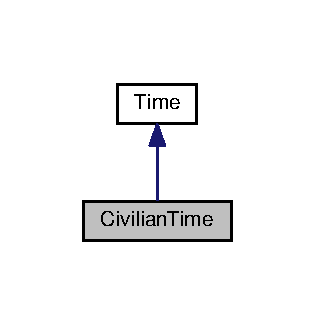
\includegraphics[width=151pt]{classCivilianTime__inherit__graph}
\end{center}
\end{figure}


Collaboration diagram for Civilian\+Time\+:
\nopagebreak
\begin{figure}[H]
\begin{center}
\leavevmode
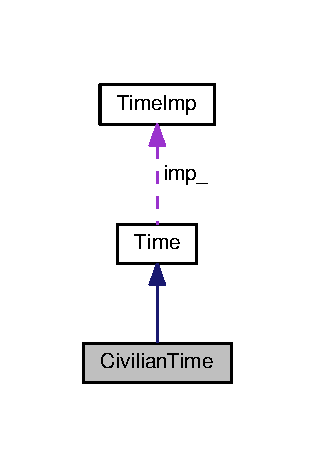
\includegraphics[width=151pt]{classCivilianTime__coll__graph}
\end{center}
\end{figure}
\subsection*{Public Member Functions}
\begin{DoxyCompactItemize}
\item 
\hyperlink{classCivilianTime_abd07d3fcd877a5bfe28037075b867393}{Civilian\+Time} (int hr, int min, int pm)
\end{DoxyCompactItemize}
\subsection*{Additional Inherited Members}


\subsection{Constructor \& Destructor Documentation}
\index{Civilian\+Time@{Civilian\+Time}!Civilian\+Time@{Civilian\+Time}}
\index{Civilian\+Time@{Civilian\+Time}!Civilian\+Time@{Civilian\+Time}}
\subsubsection[{\texorpdfstring{Civilian\+Time(int hr, int min, int pm)}{CivilianTime(int hr, int min, int pm)}}]{\setlength{\rightskip}{0pt plus 5cm}Civilian\+Time\+::\+Civilian\+Time (
\begin{DoxyParamCaption}
\item[{int}]{hr, }
\item[{int}]{min, }
\item[{int}]{pm}
\end{DoxyParamCaption}
)\hspace{0.3cm}{\ttfamily [inline]}}\hypertarget{classCivilianTime_abd07d3fcd877a5bfe28037075b867393}{}\label{classCivilianTime_abd07d3fcd877a5bfe28037075b867393}

\begin{DoxyCode}
68                                           \{
69         \hyperlink{classTime_aff6dd04cd8d4defb86a0153c17cfe6b9}{imp\_} = \textcolor{keyword}{new} \hyperlink{classCivilianTimeImp}{CivilianTimeImp}(hr, min, pm);
70     \}
\end{DoxyCode}


The documentation for this class was generated from the following file\+:\begin{DoxyCompactItemize}
\item 
\hyperlink{BridgePattern_8cpp}{Bridge\+Pattern.\+cpp}\end{DoxyCompactItemize}

\hypertarget{classCivilianTimeImp}{}\section{Civilian\+Time\+Imp Class Reference}
\label{classCivilianTimeImp}\index{Civilian\+Time\+Imp@{Civilian\+Time\+Imp}}


Inheritance diagram for Civilian\+Time\+Imp\+:
\nopagebreak
\begin{figure}[H]
\begin{center}
\leavevmode
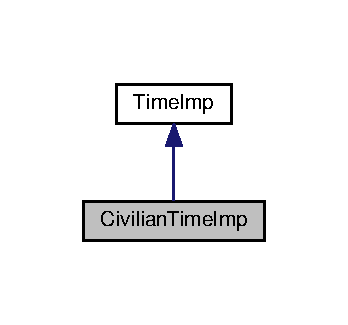
\includegraphics[width=167pt]{classCivilianTimeImp__inherit__graph}
\end{center}
\end{figure}


Collaboration diagram for Civilian\+Time\+Imp\+:
\nopagebreak
\begin{figure}[H]
\begin{center}
\leavevmode
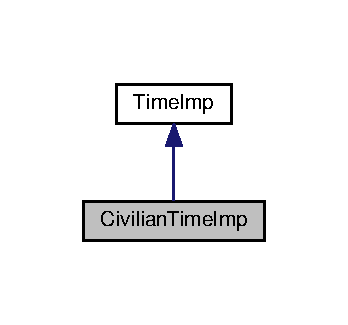
\includegraphics[width=167pt]{classCivilianTimeImp__coll__graph}
\end{center}
\end{figure}
\subsection*{Public Member Functions}
\begin{DoxyCompactItemize}
\item 
\hyperlink{classCivilianTimeImp_a81d01c53e19c0b8732b125c036c17ddb}{Civilian\+Time\+Imp} (int hr, int min, int pm)
\item 
void \hyperlink{classCivilianTimeImp_a244dd99398227e08c4e8075c85e035b3}{tell} ()
\end{DoxyCompactItemize}
\subsection*{Protected Attributes}
\begin{DoxyCompactItemize}
\item 
char \hyperlink{classCivilianTimeImp_a5d972a467fe32c2742252d34bb75a684}{which\+M\+\_\+} \mbox{[}4\mbox{]}
\end{DoxyCompactItemize}


\subsection{Constructor \& Destructor Documentation}
\index{Civilian\+Time\+Imp@{Civilian\+Time\+Imp}!Civilian\+Time\+Imp@{Civilian\+Time\+Imp}}
\index{Civilian\+Time\+Imp@{Civilian\+Time\+Imp}!Civilian\+Time\+Imp@{Civilian\+Time\+Imp}}
\subsubsection[{\texorpdfstring{Civilian\+Time\+Imp(int hr, int min, int pm)}{CivilianTimeImp(int hr, int min, int pm)}}]{\setlength{\rightskip}{0pt plus 5cm}Civilian\+Time\+Imp\+::\+Civilian\+Time\+Imp (
\begin{DoxyParamCaption}
\item[{int}]{hr, }
\item[{int}]{min, }
\item[{int}]{pm}
\end{DoxyParamCaption}
)\hspace{0.3cm}{\ttfamily [inline]}}\hypertarget{classCivilianTimeImp_a81d01c53e19c0b8732b125c036c17ddb}{}\label{classCivilianTimeImp_a81d01c53e19c0b8732b125c036c17ddb}

\begin{DoxyCode}
20                                             : \hyperlink{classTimeImp_a816d73822130c581b048e223bc0d673f}{TimeImp}(hr, min) \{
21         \textcolor{keywordflow}{if} (pm)
22           strcpy(\hyperlink{classCivilianTimeImp_a5d972a467fe32c2742252d34bb75a684}{whichM\_}, \textcolor{stringliteral}{" PM"});
23         \textcolor{keywordflow}{else}
24           strcpy(\hyperlink{classCivilianTimeImp_a5d972a467fe32c2742252d34bb75a684}{whichM\_}, \textcolor{stringliteral}{" AM"});
25     \}
\end{DoxyCode}


\subsection{Member Function Documentation}
\index{Civilian\+Time\+Imp@{Civilian\+Time\+Imp}!tell@{tell}}
\index{tell@{tell}!Civilian\+Time\+Imp@{Civilian\+Time\+Imp}}
\subsubsection[{\texorpdfstring{tell()}{tell()}}]{\setlength{\rightskip}{0pt plus 5cm}void Civilian\+Time\+Imp\+::tell (
\begin{DoxyParamCaption}
{}
\end{DoxyParamCaption}
)\hspace{0.3cm}{\ttfamily [inline]}, {\ttfamily [virtual]}}\hypertarget{classCivilianTimeImp_a244dd99398227e08c4e8075c85e035b3}{}\label{classCivilianTimeImp_a244dd99398227e08c4e8075c85e035b3}


Reimplemented from \hyperlink{classTimeImp_a266929eda5b78be282a9872b7785557b}{Time\+Imp}.


\begin{DoxyCode}
28                 \{
29         cout << \textcolor{stringliteral}{"time is "} << \hyperlink{classTimeImp_aa4d75bb67cdab3e797171e78996ac551}{hr\_} << \textcolor{stringliteral}{":"} << \hyperlink{classTimeImp_a72b908ae45367b24517a769ec9bb613f}{min\_} << \hyperlink{classCivilianTimeImp_a5d972a467fe32c2742252d34bb75a684}{whichM\_} << endl;
30     \}
\end{DoxyCode}


\subsection{Member Data Documentation}
\index{Civilian\+Time\+Imp@{Civilian\+Time\+Imp}!which\+M\+\_\+@{which\+M\+\_\+}}
\index{which\+M\+\_\+@{which\+M\+\_\+}!Civilian\+Time\+Imp@{Civilian\+Time\+Imp}}
\subsubsection[{\texorpdfstring{which\+M\+\_\+}{whichM_}}]{\setlength{\rightskip}{0pt plus 5cm}char Civilian\+Time\+Imp\+::which\+M\+\_\+\mbox{[}4\mbox{]}\hspace{0.3cm}{\ttfamily [protected]}}\hypertarget{classCivilianTimeImp_a5d972a467fe32c2742252d34bb75a684}{}\label{classCivilianTimeImp_a5d972a467fe32c2742252d34bb75a684}


The documentation for this class was generated from the following file\+:\begin{DoxyCompactItemize}
\item 
\hyperlink{BridgePattern_8cpp}{Bridge\+Pattern.\+cpp}\end{DoxyCompactItemize}

\hypertarget{classTime}{}\section{Time Class Reference}
\label{classTime}\index{Time@{Time}}


{\ttfamily \#include $<$Time.\+h$>$}

\subsection*{Public Member Functions}
\begin{DoxyCompactItemize}
\item 
\hyperlink{classTime_a0fc29d4a1be77a0f9fe1cd28c1d34958}{Time} (int h=0, int m=0, int s=0)
\item 
int \hyperlink{classTime_a4e9d93c2aaaac84b0a49f44184968860}{get\+Hour} () const 
\item 
void \hyperlink{classTime_a79e74e17893cf244e1318ceb9b1c7f32}{set\+Hour} (int h)
\item 
int \hyperlink{classTime_a6ccac73be7aacc12410cea6b3d216357}{get\+Minute} () const 
\item 
void \hyperlink{classTime_a35779c16a9db3499a27eccd58793f3b5}{set\+Minute} (int m)
\item 
int \hyperlink{classTime_adc2217366bfc4bb39eb547982747b6da}{get\+Second} () const 
\item 
void \hyperlink{classTime_a0528cf12858546b60ebb33fdcbc3fca2}{set\+Second} (int s)
\item 
void \hyperlink{classTime_ae05f94882a72debabb02e0889054d89a}{set\+Time} (int h, int m, int s)
\item 
void \hyperlink{classTime_acd9b7522e50fc667d81468219c5756e8}{print} () const 
\item 
void \hyperlink{classTime_a888a02dc15e919c5bafc4dcc95f093b7}{next\+Second} ()
\end{DoxyCompactItemize}
\subsection*{Private Attributes}
\begin{DoxyCompactItemize}
\item 
int \hyperlink{classTime_a497d35aa44ea40706dbab08f7a31d069}{hour}
\item 
int \hyperlink{classTime_a6c2e13147da34803a9784aa2b8bf8da8}{minute}
\item 
int \hyperlink{classTime_a63c9e64c7b453e10ba0f7f28bfedbcbf}{second}
\end{DoxyCompactItemize}


\subsection{Constructor \& Destructor Documentation}
\index{Time@{Time}!Time@{Time}}
\index{Time@{Time}!Time@{Time}}
\subsubsection[{\texorpdfstring{Time(int h=0, int m=0, int s=0)}{Time(int h=0, int m=0, int s=0)}}]{\setlength{\rightskip}{0pt plus 5cm}Time\+::\+Time (
\begin{DoxyParamCaption}
\item[{int}]{h = {\ttfamily 0}, }
\item[{int}]{m = {\ttfamily 0}, }
\item[{int}]{s = {\ttfamily 0}}
\end{DoxyParamCaption}
)}\hypertarget{classTime_a0fc29d4a1be77a0f9fe1cd28c1d34958}{}\label{classTime_a0fc29d4a1be77a0f9fe1cd28c1d34958}

\begin{DoxyCode}
8                               \{
9    \hyperlink{classTime_a497d35aa44ea40706dbab08f7a31d069}{hour} = h;
10    \hyperlink{classTime_a6c2e13147da34803a9784aa2b8bf8da8}{minute} = m;
11    \hyperlink{classTime_a63c9e64c7b453e10ba0f7f28bfedbcbf}{second} = s;
12 \}
\end{DoxyCode}


\subsection{Member Function Documentation}
\index{Time@{Time}!get\+Hour@{get\+Hour}}
\index{get\+Hour@{get\+Hour}!Time@{Time}}
\subsubsection[{\texorpdfstring{get\+Hour() const }{getHour() const }}]{\setlength{\rightskip}{0pt plus 5cm}int Time\+::get\+Hour (
\begin{DoxyParamCaption}
{}
\end{DoxyParamCaption}
) const}\hypertarget{classTime_a4e9d93c2aaaac84b0a49f44184968860}{}\label{classTime_a4e9d93c2aaaac84b0a49f44184968860}

\begin{DoxyCode}
15                         \{
16    \textcolor{keywordflow}{return} \hyperlink{classTime_a497d35aa44ea40706dbab08f7a31d069}{hour};
17 \}
\end{DoxyCode}
\index{Time@{Time}!get\+Minute@{get\+Minute}}
\index{get\+Minute@{get\+Minute}!Time@{Time}}
\subsubsection[{\texorpdfstring{get\+Minute() const }{getMinute() const }}]{\setlength{\rightskip}{0pt plus 5cm}int Time\+::get\+Minute (
\begin{DoxyParamCaption}
{}
\end{DoxyParamCaption}
) const}\hypertarget{classTime_a6ccac73be7aacc12410cea6b3d216357}{}\label{classTime_a6ccac73be7aacc12410cea6b3d216357}

\begin{DoxyCode}
25                           \{
26    \textcolor{keywordflow}{return} \hyperlink{classTime_a6c2e13147da34803a9784aa2b8bf8da8}{minute};
27 \}
\end{DoxyCode}
\index{Time@{Time}!get\+Second@{get\+Second}}
\index{get\+Second@{get\+Second}!Time@{Time}}
\subsubsection[{\texorpdfstring{get\+Second() const }{getSecond() const }}]{\setlength{\rightskip}{0pt plus 5cm}int Time\+::get\+Second (
\begin{DoxyParamCaption}
{}
\end{DoxyParamCaption}
) const}\hypertarget{classTime_adc2217366bfc4bb39eb547982747b6da}{}\label{classTime_adc2217366bfc4bb39eb547982747b6da}

\begin{DoxyCode}
35                           \{
36    \textcolor{keywordflow}{return} \hyperlink{classTime_a63c9e64c7b453e10ba0f7f28bfedbcbf}{second};
37 \}
\end{DoxyCode}
\index{Time@{Time}!next\+Second@{next\+Second}}
\index{next\+Second@{next\+Second}!Time@{Time}}
\subsubsection[{\texorpdfstring{next\+Second()}{nextSecond()}}]{\setlength{\rightskip}{0pt plus 5cm}void Time\+::next\+Second (
\begin{DoxyParamCaption}
{}
\end{DoxyParamCaption}
)}\hypertarget{classTime_a888a02dc15e919c5bafc4dcc95f093b7}{}\label{classTime_a888a02dc15e919c5bafc4dcc95f093b7}

\begin{DoxyCode}
60                       \{
61    ++\hyperlink{classTime_a63c9e64c7b453e10ba0f7f28bfedbcbf}{second};
62    \textcolor{keywordflow}{if} (\hyperlink{classTime_a63c9e64c7b453e10ba0f7f28bfedbcbf}{second} >= 60) \{
63       \hyperlink{classTime_a0528cf12858546b60ebb33fdcbc3fca2}{setSecond}(0);
64       \hyperlink{classTime_a35779c16a9db3499a27eccd58793f3b5}{setMinute}(++\hyperlink{classTime_a6c2e13147da34803a9784aa2b8bf8da8}{minute});
65    \}
66    \textcolor{keywordflow}{if} (\hyperlink{classTime_a6c2e13147da34803a9784aa2b8bf8da8}{minute} >= 60) \{
67       \hyperlink{classTime_a35779c16a9db3499a27eccd58793f3b5}{setMinute}(0);
68       \hyperlink{classTime_a79e74e17893cf244e1318ceb9b1c7f32}{setHour}(++\hyperlink{classTime_a497d35aa44ea40706dbab08f7a31d069}{hour});
69    \}
70    \textcolor{keywordflow}{if} (\hyperlink{classTime_a497d35aa44ea40706dbab08f7a31d069}{hour} >= 24) \{
71       \hyperlink{classTime_a79e74e17893cf244e1318ceb9b1c7f32}{setHour}(0);
72    \}
73 \}\end{DoxyCode}
\index{Time@{Time}!print@{print}}
\index{print@{print}!Time@{Time}}
\subsubsection[{\texorpdfstring{print() const }{print() const }}]{\setlength{\rightskip}{0pt plus 5cm}void Time\+::print (
\begin{DoxyParamCaption}
{}
\end{DoxyParamCaption}
) const}\hypertarget{classTime_acd9b7522e50fc667d81468219c5756e8}{}\label{classTime_acd9b7522e50fc667d81468219c5756e8}

\begin{DoxyCode}
52                        \{
53    cout << setfill(\textcolor{charliteral}{'0'});    \textcolor{comment}{// zero-filled, need <iomanip>, sticky}
54    cout << setw(2) << \hyperlink{classTime_a497d35aa44ea40706dbab08f7a31d069}{hour}  \textcolor{comment}{// set width to 2 spaces, need <iomanip>, non-sticky}
55         << \textcolor{stringliteral}{":"} << setw(2) << \hyperlink{classTime_a6c2e13147da34803a9784aa2b8bf8da8}{minute}
56         << \textcolor{stringliteral}{":"} << setw(2) << \hyperlink{classTime_a63c9e64c7b453e10ba0f7f28bfedbcbf}{second} << endl;
57 \}
\end{DoxyCode}
\index{Time@{Time}!set\+Hour@{set\+Hour}}
\index{set\+Hour@{set\+Hour}!Time@{Time}}
\subsubsection[{\texorpdfstring{set\+Hour(int h)}{setHour(int h)}}]{\setlength{\rightskip}{0pt plus 5cm}void Time\+::set\+Hour (
\begin{DoxyParamCaption}
\item[{int}]{h}
\end{DoxyParamCaption}
)}\hypertarget{classTime_a79e74e17893cf244e1318ceb9b1c7f32}{}\label{classTime_a79e74e17893cf244e1318ceb9b1c7f32}

\begin{DoxyCode}
20                         \{
21    \hyperlink{classTime_a497d35aa44ea40706dbab08f7a31d069}{hour} = h;
22 \}
\end{DoxyCode}
\index{Time@{Time}!set\+Minute@{set\+Minute}}
\index{set\+Minute@{set\+Minute}!Time@{Time}}
\subsubsection[{\texorpdfstring{set\+Minute(int m)}{setMinute(int m)}}]{\setlength{\rightskip}{0pt plus 5cm}void Time\+::set\+Minute (
\begin{DoxyParamCaption}
\item[{int}]{m}
\end{DoxyParamCaption}
)}\hypertarget{classTime_a35779c16a9db3499a27eccd58793f3b5}{}\label{classTime_a35779c16a9db3499a27eccd58793f3b5}

\begin{DoxyCode}
30                           \{
31    \hyperlink{classTime_a6c2e13147da34803a9784aa2b8bf8da8}{minute} = m;
32 \}
\end{DoxyCode}
\index{Time@{Time}!set\+Second@{set\+Second}}
\index{set\+Second@{set\+Second}!Time@{Time}}
\subsubsection[{\texorpdfstring{set\+Second(int s)}{setSecond(int s)}}]{\setlength{\rightskip}{0pt plus 5cm}void Time\+::set\+Second (
\begin{DoxyParamCaption}
\item[{int}]{s}
\end{DoxyParamCaption}
)}\hypertarget{classTime_a0528cf12858546b60ebb33fdcbc3fca2}{}\label{classTime_a0528cf12858546b60ebb33fdcbc3fca2}

\begin{DoxyCode}
40                           \{
41    \hyperlink{classTime_a63c9e64c7b453e10ba0f7f28bfedbcbf}{second} = s;
42 \}
\end{DoxyCode}
\index{Time@{Time}!set\+Time@{set\+Time}}
\index{set\+Time@{set\+Time}!Time@{Time}}
\subsubsection[{\texorpdfstring{set\+Time(int h, int m, int s)}{setTime(int h, int m, int s)}}]{\setlength{\rightskip}{0pt plus 5cm}void Time\+::set\+Time (
\begin{DoxyParamCaption}
\item[{int}]{h, }
\item[{int}]{m, }
\item[{int}]{s}
\end{DoxyParamCaption}
)}\hypertarget{classTime_ae05f94882a72debabb02e0889054d89a}{}\label{classTime_ae05f94882a72debabb02e0889054d89a}

\begin{DoxyCode}
45                                       \{
46    \hyperlink{classTime_a79e74e17893cf244e1318ceb9b1c7f32}{setHour}(h);
47    \hyperlink{classTime_a35779c16a9db3499a27eccd58793f3b5}{setMinute}(m);
48    \hyperlink{classTime_a0528cf12858546b60ebb33fdcbc3fca2}{setSecond}(s);
49 \}
\end{DoxyCode}


\subsection{Member Data Documentation}
\index{Time@{Time}!hour@{hour}}
\index{hour@{hour}!Time@{Time}}
\subsubsection[{\texorpdfstring{hour}{hour}}]{\setlength{\rightskip}{0pt plus 5cm}int Time\+::hour\hspace{0.3cm}{\ttfamily [private]}}\hypertarget{classTime_a497d35aa44ea40706dbab08f7a31d069}{}\label{classTime_a497d35aa44ea40706dbab08f7a31d069}
\index{Time@{Time}!minute@{minute}}
\index{minute@{minute}!Time@{Time}}
\subsubsection[{\texorpdfstring{minute}{minute}}]{\setlength{\rightskip}{0pt plus 5cm}int Time\+::minute\hspace{0.3cm}{\ttfamily [private]}}\hypertarget{classTime_a6c2e13147da34803a9784aa2b8bf8da8}{}\label{classTime_a6c2e13147da34803a9784aa2b8bf8da8}
\index{Time@{Time}!second@{second}}
\index{second@{second}!Time@{Time}}
\subsubsection[{\texorpdfstring{second}{second}}]{\setlength{\rightskip}{0pt plus 5cm}int Time\+::second\hspace{0.3cm}{\ttfamily [private]}}\hypertarget{classTime_a63c9e64c7b453e10ba0f7f28bfedbcbf}{}\label{classTime_a63c9e64c7b453e10ba0f7f28bfedbcbf}


The documentation for this class was generated from the following files\+:\begin{DoxyCompactItemize}
\item 
\hyperlink{Time_8h}{Time.\+h}\item 
\hyperlink{Time_8cpp}{Time.\+cpp}\end{DoxyCompactItemize}

\hypertarget{classTimeImp}{}\section{Time\+Imp Class Reference}
\label{classTimeImp}\index{Time\+Imp@{Time\+Imp}}


Inheritance diagram for Time\+Imp\+:
\nopagebreak
\begin{figure}[H]
\begin{center}
\leavevmode
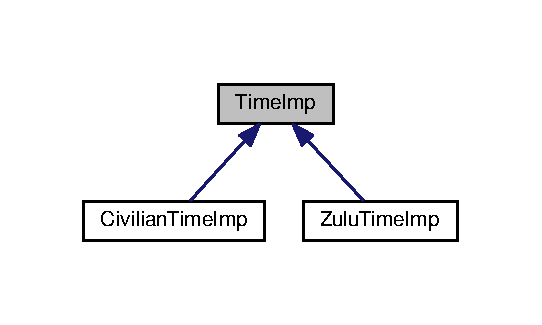
\includegraphics[width=260pt]{classTimeImp__inherit__graph}
\end{center}
\end{figure}
\subsection*{Public Member Functions}
\begin{DoxyCompactItemize}
\item 
\hyperlink{classTimeImp_a816d73822130c581b048e223bc0d673f}{Time\+Imp} (int hr, int min)
\item 
virtual void \hyperlink{classTimeImp_a266929eda5b78be282a9872b7785557b}{tell} ()
\end{DoxyCompactItemize}
\subsection*{Protected Attributes}
\begin{DoxyCompactItemize}
\item 
int \hyperlink{classTimeImp_aa4d75bb67cdab3e797171e78996ac551}{hr\+\_\+}
\item 
int \hyperlink{classTimeImp_a72b908ae45367b24517a769ec9bb613f}{min\+\_\+}
\end{DoxyCompactItemize}


\subsection{Constructor \& Destructor Documentation}
\index{Time\+Imp@{Time\+Imp}!Time\+Imp@{Time\+Imp}}
\index{Time\+Imp@{Time\+Imp}!Time\+Imp@{Time\+Imp}}
\subsubsection[{\texorpdfstring{Time\+Imp(int hr, int min)}{TimeImp(int hr, int min)}}]{\setlength{\rightskip}{0pt plus 5cm}Time\+Imp\+::\+Time\+Imp (
\begin{DoxyParamCaption}
\item[{int}]{hr, }
\item[{int}]{min}
\end{DoxyParamCaption}
)\hspace{0.3cm}{\ttfamily [inline]}}\hypertarget{classTimeImp_a816d73822130c581b048e223bc0d673f}{}\label{classTimeImp_a816d73822130c581b048e223bc0d673f}

\begin{DoxyCode}
7                              \{
8         \hyperlink{classTimeImp_aa4d75bb67cdab3e797171e78996ac551}{hr\_} = hr;
9         \hyperlink{classTimeImp_a72b908ae45367b24517a769ec9bb613f}{min\_} = min;
10     \}
\end{DoxyCode}


\subsection{Member Function Documentation}
\index{Time\+Imp@{Time\+Imp}!tell@{tell}}
\index{tell@{tell}!Time\+Imp@{Time\+Imp}}
\subsubsection[{\texorpdfstring{tell()}{tell()}}]{\setlength{\rightskip}{0pt plus 5cm}virtual void Time\+Imp\+::tell (
\begin{DoxyParamCaption}
{}
\end{DoxyParamCaption}
)\hspace{0.3cm}{\ttfamily [inline]}, {\ttfamily [virtual]}}\hypertarget{classTimeImp_a266929eda5b78be282a9872b7785557b}{}\label{classTimeImp_a266929eda5b78be282a9872b7785557b}


Reimplemented in \hyperlink{classZuluTimeImp_ac7b726f1341e591e346240327dd8bbd1}{Zulu\+Time\+Imp}, and \hyperlink{classCivilianTimeImp_a244dd99398227e08c4e8075c85e035b3}{Civilian\+Time\+Imp}.


\begin{DoxyCode}
11                         \{
12         cout << \textcolor{stringliteral}{"time is "} << setw(2) << setfill(48) << \hyperlink{classTimeImp_aa4d75bb67cdab3e797171e78996ac551}{hr\_} << \hyperlink{classTimeImp_a72b908ae45367b24517a769ec9bb613f}{min\_} << endl;
13     \}
\end{DoxyCode}


\subsection{Member Data Documentation}
\index{Time\+Imp@{Time\+Imp}!hr\+\_\+@{hr\+\_\+}}
\index{hr\+\_\+@{hr\+\_\+}!Time\+Imp@{Time\+Imp}}
\subsubsection[{\texorpdfstring{hr\+\_\+}{hr_}}]{\setlength{\rightskip}{0pt plus 5cm}int Time\+Imp\+::hr\+\_\+\hspace{0.3cm}{\ttfamily [protected]}}\hypertarget{classTimeImp_aa4d75bb67cdab3e797171e78996ac551}{}\label{classTimeImp_aa4d75bb67cdab3e797171e78996ac551}
\index{Time\+Imp@{Time\+Imp}!min\+\_\+@{min\+\_\+}}
\index{min\+\_\+@{min\+\_\+}!Time\+Imp@{Time\+Imp}}
\subsubsection[{\texorpdfstring{min\+\_\+}{min_}}]{\setlength{\rightskip}{0pt plus 5cm}int Time\+Imp\+::min\+\_\+\hspace{0.3cm}{\ttfamily [protected]}}\hypertarget{classTimeImp_a72b908ae45367b24517a769ec9bb613f}{}\label{classTimeImp_a72b908ae45367b24517a769ec9bb613f}


The documentation for this class was generated from the following file\+:\begin{DoxyCompactItemize}
\item 
\hyperlink{BridgePattern_8cpp}{Bridge\+Pattern.\+cpp}\end{DoxyCompactItemize}

\hypertarget{classZuluTime}{}\section{Zulu\+Time Class Reference}
\label{classZuluTime}\index{Zulu\+Time@{Zulu\+Time}}


Inheritance diagram for Zulu\+Time\+:
\nopagebreak
\begin{figure}[H]
\begin{center}
\leavevmode
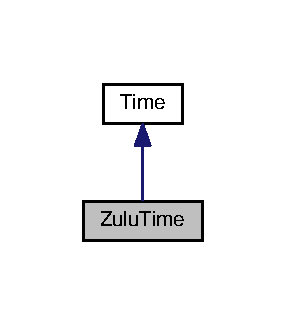
\includegraphics[width=137pt]{classZuluTime__inherit__graph}
\end{center}
\end{figure}


Collaboration diagram for Zulu\+Time\+:
\nopagebreak
\begin{figure}[H]
\begin{center}
\leavevmode
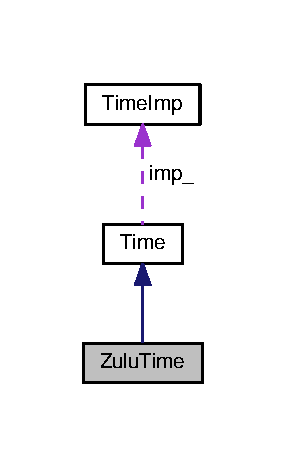
\includegraphics[width=137pt]{classZuluTime__coll__graph}
\end{center}
\end{figure}
\subsection*{Public Member Functions}
\begin{DoxyCompactItemize}
\item 
\hyperlink{classZuluTime_a8e9a19871eaca29ea45a3154b388c27a}{Zulu\+Time} (int hr, int min, int zone)
\end{DoxyCompactItemize}
\subsection*{Additional Inherited Members}


\subsection{Constructor \& Destructor Documentation}
\index{Zulu\+Time@{Zulu\+Time}!Zulu\+Time@{Zulu\+Time}}
\index{Zulu\+Time@{Zulu\+Time}!Zulu\+Time@{Zulu\+Time}}
\subsubsection[{\texorpdfstring{Zulu\+Time(int hr, int min, int zone)}{ZuluTime(int hr, int min, int zone)}}]{\setlength{\rightskip}{0pt plus 5cm}Zulu\+Time\+::\+Zulu\+Time (
\begin{DoxyParamCaption}
\item[{int}]{hr, }
\item[{int}]{min, }
\item[{int}]{zone}
\end{DoxyParamCaption}
)\hspace{0.3cm}{\ttfamily [inline]}}\hypertarget{classZuluTime_a8e9a19871eaca29ea45a3154b388c27a}{}\label{classZuluTime_a8e9a19871eaca29ea45a3154b388c27a}

\begin{DoxyCode}
75                                         \{
76         \hyperlink{classTime_aff6dd04cd8d4defb86a0153c17cfe6b9}{imp\_} = \textcolor{keyword}{new} \hyperlink{classZuluTimeImp}{ZuluTimeImp}(hr, min, zone);
77     \}
\end{DoxyCode}


The documentation for this class was generated from the following file\+:\begin{DoxyCompactItemize}
\item 
\hyperlink{BridgePattern_8cpp}{Bridge\+Pattern.\+cpp}\end{DoxyCompactItemize}

\hypertarget{classZuluTimeImp}{}\section{Zulu\+Time\+Imp Class Reference}
\label{classZuluTimeImp}\index{Zulu\+Time\+Imp@{Zulu\+Time\+Imp}}


Inheritance diagram for Zulu\+Time\+Imp\+:
\nopagebreak
\begin{figure}[H]
\begin{center}
\leavevmode
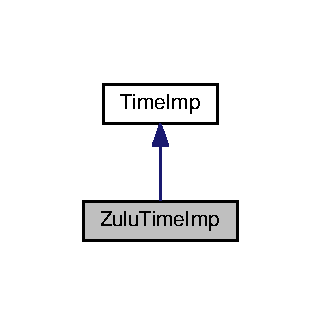
\includegraphics[width=154pt]{classZuluTimeImp__inherit__graph}
\end{center}
\end{figure}


Collaboration diagram for Zulu\+Time\+Imp\+:
\nopagebreak
\begin{figure}[H]
\begin{center}
\leavevmode
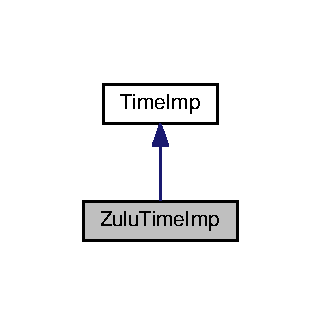
\includegraphics[width=154pt]{classZuluTimeImp__coll__graph}
\end{center}
\end{figure}
\subsection*{Public Member Functions}
\begin{DoxyCompactItemize}
\item 
\hyperlink{classZuluTimeImp_af75d85b608a7d4d783e46d868aee841c}{Zulu\+Time\+Imp} (int hr, int min, int zone)
\item 
void \hyperlink{classZuluTimeImp_ac7b726f1341e591e346240327dd8bbd1}{tell} ()
\end{DoxyCompactItemize}
\subsection*{Protected Attributes}
\begin{DoxyCompactItemize}
\item 
char \hyperlink{classZuluTimeImp_a1fd091e92c79ccf25066c6f016f7892d}{zone\+\_\+} \mbox{[}30\mbox{]}
\end{DoxyCompactItemize}


\subsection{Constructor \& Destructor Documentation}
\index{Zulu\+Time\+Imp@{Zulu\+Time\+Imp}!Zulu\+Time\+Imp@{Zulu\+Time\+Imp}}
\index{Zulu\+Time\+Imp@{Zulu\+Time\+Imp}!Zulu\+Time\+Imp@{Zulu\+Time\+Imp}}
\subsubsection[{\texorpdfstring{Zulu\+Time\+Imp(int hr, int min, int zone)}{ZuluTimeImp(int hr, int min, int zone)}}]{\setlength{\rightskip}{0pt plus 5cm}Zulu\+Time\+Imp\+::\+Zulu\+Time\+Imp (
\begin{DoxyParamCaption}
\item[{int}]{hr, }
\item[{int}]{min, }
\item[{int}]{zone}
\end{DoxyParamCaption}
)\hspace{0.3cm}{\ttfamily [inline]}}\hypertarget{classZuluTimeImp_af75d85b608a7d4d783e46d868aee841c}{}\label{classZuluTimeImp_af75d85b608a7d4d783e46d868aee841c}

\begin{DoxyCode}
37                                           : \hyperlink{classTimeImp_a816d73822130c581b048e223bc0d673f}{TimeImp}(hr, min) \{
38         \textcolor{keywordflow}{if} (zone == 5)
39           strcpy(\hyperlink{classZuluTimeImp_a1fd091e92c79ccf25066c6f016f7892d}{zone\_}, \textcolor{stringliteral}{" Eastern Standard Time"});
40         \textcolor{keywordflow}{else} \textcolor{keywordflow}{if} (zone == 6)
41           strcpy(\hyperlink{classZuluTimeImp_a1fd091e92c79ccf25066c6f016f7892d}{zone\_}, \textcolor{stringliteral}{" Central Standard Time"});
42     \}
\end{DoxyCode}


\subsection{Member Function Documentation}
\index{Zulu\+Time\+Imp@{Zulu\+Time\+Imp}!tell@{tell}}
\index{tell@{tell}!Zulu\+Time\+Imp@{Zulu\+Time\+Imp}}
\subsubsection[{\texorpdfstring{tell()}{tell()}}]{\setlength{\rightskip}{0pt plus 5cm}void Zulu\+Time\+Imp\+::tell (
\begin{DoxyParamCaption}
{}
\end{DoxyParamCaption}
)\hspace{0.3cm}{\ttfamily [inline]}, {\ttfamily [virtual]}}\hypertarget{classZuluTimeImp_ac7b726f1341e591e346240327dd8bbd1}{}\label{classZuluTimeImp_ac7b726f1341e591e346240327dd8bbd1}


Reimplemented from \hyperlink{classTimeImp_a266929eda5b78be282a9872b7785557b}{Time\+Imp}.


\begin{DoxyCode}
45                 \{
46         cout << \textcolor{stringliteral}{"time is "} << setw(2) << setfill(48) << \hyperlink{classTimeImp_aa4d75bb67cdab3e797171e78996ac551}{hr\_} << \hyperlink{classTimeImp_a72b908ae45367b24517a769ec9bb613f}{min\_} << 
      \hyperlink{classZuluTimeImp_a1fd091e92c79ccf25066c6f016f7892d}{zone\_} <<
47           endl;
48     \}
\end{DoxyCode}


\subsection{Member Data Documentation}
\index{Zulu\+Time\+Imp@{Zulu\+Time\+Imp}!zone\+\_\+@{zone\+\_\+}}
\index{zone\+\_\+@{zone\+\_\+}!Zulu\+Time\+Imp@{Zulu\+Time\+Imp}}
\subsubsection[{\texorpdfstring{zone\+\_\+}{zone_}}]{\setlength{\rightskip}{0pt plus 5cm}char Zulu\+Time\+Imp\+::zone\+\_\+\mbox{[}30\mbox{]}\hspace{0.3cm}{\ttfamily [protected]}}\hypertarget{classZuluTimeImp_a1fd091e92c79ccf25066c6f016f7892d}{}\label{classZuluTimeImp_a1fd091e92c79ccf25066c6f016f7892d}


The documentation for this class was generated from the following file\+:\begin{DoxyCompactItemize}
\item 
\hyperlink{BridgePattern_8cpp}{Bridge\+Pattern.\+cpp}\end{DoxyCompactItemize}

\chapter{File Documentation}
\hypertarget{BridgePattern_8cpp}{}\section{Bridge\+Pattern.\+cpp File Reference}
\label{BridgePattern_8cpp}\index{Bridge\+Pattern.\+cpp@{Bridge\+Pattern.\+cpp}}
{\ttfamily \#include $<$iostream.\+h$>$}\\*
{\ttfamily \#include $<$iomanip.\+h$>$}\\*
{\ttfamily \#include $<$string.\+h$>$}\\*
Include dependency graph for Bridge\+Pattern.\+cpp\+:
\nopagebreak
\begin{figure}[H]
\begin{center}
\leavevmode
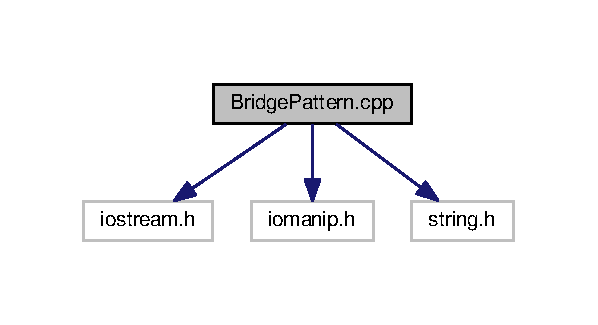
\includegraphics[width=287pt]{BridgePattern_8cpp__incl}
\end{center}
\end{figure}
\subsection*{Classes}
\begin{DoxyCompactItemize}
\item 
class \hyperlink{classTimeImp}{Time\+Imp}
\item 
class \hyperlink{classCivilianTimeImp}{Civilian\+Time\+Imp}
\item 
class \hyperlink{classZuluTimeImp}{Zulu\+Time\+Imp}
\item 
class \hyperlink{classTime}{Time}
\item 
class \hyperlink{classCivilianTime}{Civilian\+Time}
\item 
class \hyperlink{classZuluTime}{Zulu\+Time}
\end{DoxyCompactItemize}
\subsection*{Functions}
\begin{DoxyCompactItemize}
\item 
int \hyperlink{BridgePattern_8cpp_ae66f6b31b5ad750f1fe042a706a4e3d4}{main} ()
\end{DoxyCompactItemize}


\subsection{Function Documentation}
\index{Bridge\+Pattern.\+cpp@{Bridge\+Pattern.\+cpp}!main@{main}}
\index{main@{main}!Bridge\+Pattern.\+cpp@{Bridge\+Pattern.\+cpp}}
\subsubsection[{\texorpdfstring{main()}{main()}}]{\setlength{\rightskip}{0pt plus 5cm}int main (
\begin{DoxyParamCaption}
{}
\end{DoxyParamCaption}
)}\hypertarget{BridgePattern_8cpp_ae66f6b31b5ad750f1fe042a706a4e3d4}{}\label{BridgePattern_8cpp_ae66f6b31b5ad750f1fe042a706a4e3d4}

\begin{DoxyCode}
80            \{
81   \hyperlink{classTime}{Time} *times[3];
82   times[0] = \textcolor{keyword}{new} \hyperlink{classTime}{Time}(14, 30);
83   times[1] = \textcolor{keyword}{new} \hyperlink{classCivilianTime}{CivilianTime}(2, 30, 1);
84   times[2] = \textcolor{keyword}{new} \hyperlink{classZuluTime}{ZuluTime}(14, 30, 6);
85   \textcolor{keywordflow}{for} (\textcolor{keywordtype}{int} i = 0; i < 3; i++)
86     times[i]->tell();
87 \}\end{DoxyCode}


Here is the call graph for this function\+:
\nopagebreak
\begin{figure}[H]
\begin{center}
\leavevmode
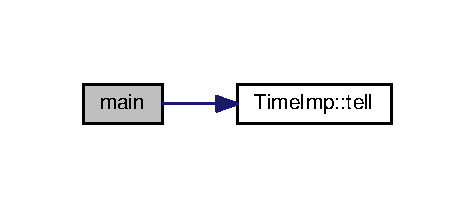
\includegraphics[width=228pt]{BridgePattern_8cpp_ae66f6b31b5ad750f1fe042a706a4e3d4_cgraph}
\end{center}
\end{figure}



%--- End generated contents ---

% Index
\backmatter
\newpage
\phantomsection
\clearemptydoublepage
\addcontentsline{toc}{chapter}{Index}
\printindex

\end{document}
